\section{Einleitung}
\subsection{Relevanz des Themas}
Um im Rahmen der globalen Ausweitung wettbewerbsfähig zu bleiben, müssen sich Unternehmen ständig auf neue Herausforderungen einstellen. Dies erfordert eine hohe Reaktionsgeschwindigkeit des Managements und somit ein leistungsfähiges Berichtswesen, welches eine möglichst aktuelle Darstellung der Unternehmenslage ermöglicht. Um die Wirtschaftlichkeit zu steigern, ist es essentiell in allen Unternehmensbereichen Kosten transparent zu erfassen und senken zu können. 
Die internationalen Märkte erfordern es, diese Unternehmensanforderungen mit facettenreichen, rechtlichen Auflagen unterschiedlichster Länder in Einklang zu bringen. 
In diesem Zusammenhang werden unabhängig von der Unternehmensgröße flexible IT-Systeme benötigt, die ein optimales Unternehmenswachstum unterstützen.

Die SAP AG ist einer der weltweit führenden Anbieter für Unternehmenssoftware und gerade auf dem deutschen Markt mit Ihren Produkten für das Rechnungswesen ein bereits etablierter Standard\footnote{Vgl. \cite{Patel2009}, S. 21. f}.

\subsection{Zielsetzung und Abgrenzung}
Diese Arbeit beschäftigt sich mit des Rechnungswesen in SAP ERP. Dabei werden die bereitgestellten Systemfunktionen zur Unterstützung des Rechnungswesens im Bezug auf die Systemmodule FI und CO differenziert betrachtet.
Ziel ist es, ein Grundverständnis der betriebswirtschaftliche Theorie zu vermitteln, die wesentlichen Systemfunktionen selbst und anschließend, im Rahmen eines Student Consulting Projects, die praktisches Umsetzung im eigenen Unternehmen zu beleuchten. Diese Arbeit versteht sich als richtungsweisend und ratgebend, zur Schärfung des Praxisverständnisses von Rechnungswesen mit SAP ERP (FI, CO) und als Einstieg zur weiteren Vertiefung.



\subsection{Vorgehen}
Die Abbildung \ref{abbeinleitung} auf Seite \pageref{abbeinleitung} zeigt eine schematische Darstellung zum Aufbau der Arbeit.
\begin{figure}[htbp]
\begin{center}
%\begin{floatingfigure}[r]{0.7\textwidth}
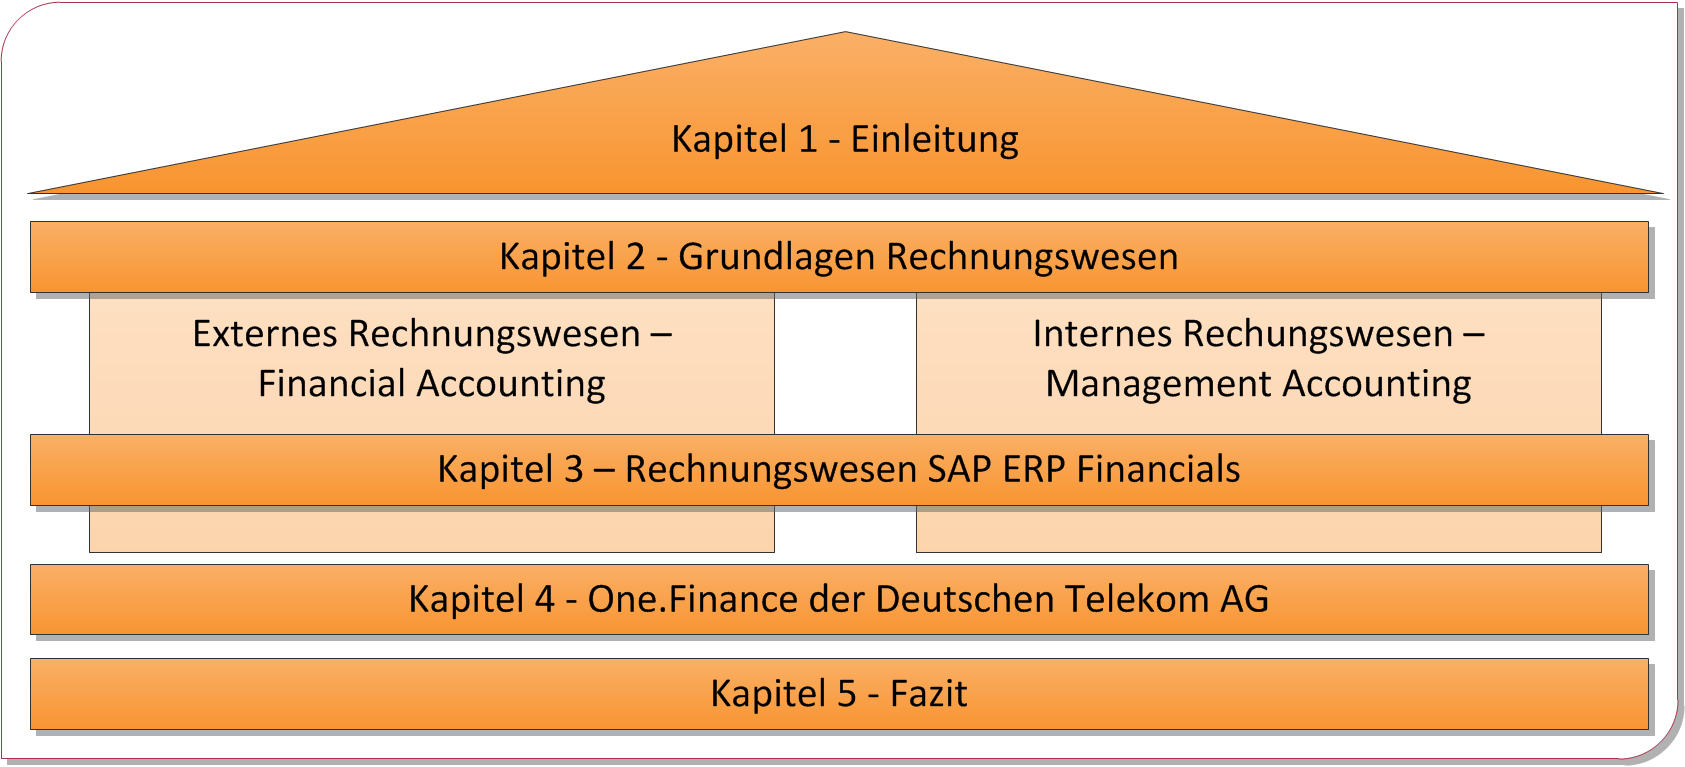
\includegraphics[width=0.8\textwidth]{Images/einleitung.png}
\caption[Aufbau dieser Arbeit]{Aufbau dieser Arbeit}
\label{abbeinleitung}
\end{center}
\end{figure}
\begin{compactitem}
\item Kapitel 1 führt an das betrachtete Thema heran und definiert die Ziele dieser Arbeit.
\item Kapitel 2 gibt einen Überblick über die allgemeinen betriebswirtschaftlichen Grundlagen des Rechnungswesen. Dabei wird der Themenkomplex in das externe und interne Rechnungswesen unterteilt.
\item Kapitel 3 behandelt die spezifische Sicht auf die Softwarelösung ERP Financials der SAP AG mit den Modulen FI und CO.
\item Kapitel 4 beinhaltet das Student Consulting Project (SCP) mit der Betrachtung der systemtechnischen Realisierung des Rechnungswesens im Konzern Deutsche Telekom AG.
\item Kapitel 5 fasst die Bedeutung zusammen und zieht das Fazit dieser Arbeit.
\end{compactitem}
